\chapter{Technische Umsetzungen}
\label{chap:technologies}

\section{DNSSEC}
\label{sec:tec-dnssec}
DNSSEC, als eine Sammlung an IETF-Spezifikationen, erweitert DNS mit dem Ziel die Integrität und Authentizität der Ressourceneinträge sicherzustellen (\cite{Arends2005}). Dies wird über die kryptographische Signatur der Einträge erreicht. Um die Signaturen validieren zu können, wird eine Chain-Of-Trust genützt, die ihren Ankerpunkt im von der ICANN veröffentlichten DNSSEC-Root-Key besitzt. Der Umstand, dass die ICANN somit als \textit{single-point-of-trust} fungiert und somit den Grundgedanken eines verteilten Internets unterwandert ist ein schwerwiegender Kritikpunkt an DNSSEC \cite{Finch2014}. Außerdem trägt die Erhöhung der Paketgröße zur Verschlimmerung der DoS-Problematik bei (siehe Abschnitt \ref{sec:attacks-dos}). 

Des weiteren findet die Erweiterung, aufgrund der langen Entwicklungszeit, der (verglichen zum DNS-Protokoll) hohen Komplexität und dem erhöhtem administrativem Aufwand, nur wenig anklang. Seit der finalen Veröffentlichen 2005 konnten zwar 90 Prozent der TLD Betreibenden zum signieren ihrer Zonen bewegt werden, die Verbreitung signierter SLDs ist mit ca. 4 Prozent jedoch zu gering um Maßgeblich zur Sicherheit des globalen DNS beizutragen\cite{DCCommunications2018}. Zusätzlich wurde das Schutzziel der Vertraulichkeit bewusst bei der Konzeptionierung ausgeklammert. Wie in Abschnitt \ref{sec:thread-priv} beschrieben, ist der Bedarf nach einer vertraulichen Möglichkeit zur Auflösung von Namen im Internet stark angestiegen. Betrachtet man nun zusätzlich den Umstand, dass das DNSSEC Netzwerkprotokoll noch stärker als reines DNS, für DoS-Amplification genützt werden kann, ist klar warum diese Spezifikationssammlung so wenig positive Resonanz erhält\cite{Antic2014}.

\section{DNSCurve}
Aufgrund der schlechten Akzeptanz und dem fehlenden Schutz der Vertraulichkeit veröffentlichte der US-amerikanische Kryptograph Daniel J. Bernstein (auch bekannt als DJB) eine eigene Lösung namens DNSCurve. Diese dient zur Sicherstellung einer vertraulichen und authentischen Kommunikation zwischen rekursiv auflösendem Server und den autoritativen Servers. Sie baut auf dem, von DJB entwickelten, elliptische Kurven-Kryptosystem Curve25519 auf und verwendet so, im vergleich zu DNSSEC, welches RSA einsetzt, elliptic-curve-cryptography (ECC), für asymmetrische Operationen. Außerdem wird der, ebenfalls selbst entwickelte, Poly1305 message-authentication-code (MAC) für die Verschlüsselung und Echtheitsprüfung der Nachrichten eingesetzt. 

Der Einsatz von ECC sorgt, im Vergleich zu RSA, für eine signifikante Verbesserung der Performance bei der Schlüsselaushandlung, da weit kürzerer Schüssel bei gleichbleibender Sicherheit eingesetzt werden können\cite{Gupta2002}. Der in RFC7905 spezifizierten Poly1305 Algorithmus ist ebenfalls auf Geschwindigkeit, unter Einhaltung der Sicherheitsansprüche, optimiert\cite{Bernstein2005}. Somit war DNSCurve, bei dessen Veröffentlichung 2009, DNSSEC, speziell im Bereich Performance, weit überlegen. Da der höhere Leistungsansprüche der Validierung bis Heute eine starkes Argument gegen den Einsatz von DNSSEC dargestellt, wurde DNSCurve, trotz des ungewöhnlichen Algorithmen, durchaus positiv aufgenommen \cite{Henry2013}. Dies Überrascht, da DNSCurve, wie D. Kaminsky feststellt, ein konzeptionellen Problem im Bereich des \textit{Trust Establishment} Prozesses ausweißt \cite{Kaminsky2011}. 

Das Protokoll verlässt sich beim Auffinden der öffentlichen Schüssel auf einen speziellen NS-Eintrag der zu Ziel-DNS-Domäne. Da DNSCurve ohne Erweiterungen des DNS-Protokolls auskommt, wird dieser Eintrag alleinig durch dessen spezielles Format aufgefunden. Darüber hinaus wird der Schlüssel in den NS-Eintrag selbst kodiert. Ein Angreifer in aktiven MitM Position, könnte somit, durch simples Umschreiben des Eintrags, eine Kommunikation über DNSCrypt unterbinden. Selbst wenn kein Fallback zur Klartextkommunikation erfolgt, besteht noch immer die Möglichkeit, ein eigenes Schlüsselpaar zu generieren und den öffentlichen Schüssel des Ziels gegen einen eigenen zu tauschen. In der Spezifikation scheint zwar die Möglichkeit zum Aufbau einer CoT auf, da eine zentrale Vertrauensinstanz bewusst fehlt, wird diese jedoch von Kaminsky als \textit{ineffektiv} bezeichnet, da sie laut ihm keine zufriedenstellende Lösung des Problems \textit{Key Management} birgt. Es ist somit fraglich, ob DNSCurve in der Lage ist die Vertraulichkeit und Authentizität von DNS sicherzustellen.  

\section{DNSCrypt}
Zusätzlich zu DNSCurve und DNSSEC wurde 2011 das Netzwerkprotokoll DNSCrypt entwickelt. Dieses ähnelt DNSCurve im grundlegenden Aufbau insofern es die von DJB entwickelten Algorithmen Curve25519 und Poly1305 zum Schlüsselaustausch und zur Überprüfung der Nachrichten verwendet und das DNS Netzwerkprotokoll ohne weiter Modifikationen für die Kommunikation einsetzt. Der größte Unterschied liegt darin, dass DNSCrypt die Kommunikation zwischen Stub-Resolver und rekursivem DNS Server schützt. Um dies zu erreichen, werden kurzlebige Zertifikate eingesetzt, welche zur Verschlüsselung der Anfragen und Validierung der Antworten eingesetzt werden. Diese Zertifikate sind mit einem langlebigen Schüssel signiert, wobei der öffentliche Schüssel von jedem Client explizit in eine Liste an vertrauenswürdigen Schüsseln aufgenommen werden muss.\cite{Denis2016} Dies umgeht zwar die konzeptionelle Schwäche von DNSCrypt formal, ist jedoch ohne entsprechende Unterstützungsmethoden unpraktikabel. 

Eine in manchen Implementierungen verwendete Lösung nach dem \textit{Trust-on-first-use}-Prinzip (TOFU) wird als nicht zuverlässig erachtet.\cite{Wendlandt2008} Somit stellt DNSCrypt, ähnlich wie DNSCurve, zwar eine sichere  Möglichkeit zum Übertragen von DNS-Anfragen und Antworten an den auflösenden DNS Server dar, vernachlässigt jedoch ebenfalls das zentrale Thema des \textit{Schlüsselmanagements}. Eine Möglichkeit zum umgehen dieser Schwäche, stellt das nutzen der öffentlichen Browser-PKI CoT oder das etablieren eines Trusts Out-Of-Bound dar. Wird das genutzte Zertifikat zum Beispiel manuell geprüft und explizit eingespielt, dann dieses von einem möglichen Angreifer nicht mehr modifiziert werden. Werden diese Wege genützt, kann das System als ausreichend Sicher angesehen werden.

\section{DNS-over-TCP}
Eine minimalistische Lösung für die DoS und Traffic-Amplification Problematik (siehe Abschnitt \ref{sec:attacks-dos}) ist der Einsatz eines verbindungsorientierten Protokolls. Es bietet sich hier TCP an, da es bereits als mögliches Transportprotokoll im ursprünglichen Standard festgelegt wurde \cite{rfc1035}. Obwohl der als \textit{T-DNS} bezeichneter Vorschlag schon früh aufkam, wurde ihm lange keine Beachtung geschenkt. Der Zeitaufwand für das Aufbauen einer Verbindung, zusammen mit dem erhöhten Ressourcenaufwand auf der Serverseite wurde als finales Gegenargument gegen den Einsatz von T-DNS verwendet. Seit 2014 mehren sich jedoch Argumente gegen dieses Dogma. Es konnte klar feststellen werden, dass moderne Systeme durchaus in der Lage sind die erhöhten Ansprüche zu erfüllen\cite{Zhu2015}. 

\section{DNS-over-TLS}
\label{sec:tec-dot}
Das Kernproblem der DNS Security besteht in der fehlender Authentizität und Vertraulichkeit der Übertragung. Diesen Umstand hat DNS mit vielen älteren Netzwerkprotokollen gemein, speziell im Internetumfeld ist HTTP, neben DNS, eines der verbreitetsten Protokolle. Als Lösung für HTTP wurde SSL bzw. TLS festgelegt, welches, nach seiner Spezifizierung 2000, das meist genützte Transportverschlüsselungsprotokoll der TCP/IP-Suite wurde. Es liegt also die Sicherheitsschwäche von DNS ebenfalls mit TLS als Transportprotokoll zu beheben. 
Angestoßen durch die früheren Arbeiten zu T-DNS, wurde das anbieten von DNS über TLS (DNS-over-TLS; DoT) im IETF Dokumenten RFC7858\cite{rfc7858} und RFC8310\cite{Dickinson2018} spezifiziert und ist sein 2016 als sichere Transportmethode zwischen 2 DNS-Endpunkten akzeptiert. Die Aufgabe der Authentifizierung wurde auf das TLS Protokoll übertragen und folgt damit den selben Mechanismen die schon von HTTPS bekannt sind. Die über ein X509 Zertifikat authentisierende Gegenstelle wird im Zuge des TLS-Handshake über vorinstallierte Stammzertifikate von Zertifizierungsstellen authentifiziert. Die Vertrauensstellung zu den Zielservern ist daher, wie bei HTTPS, implizit transitiv über das Vertrauen zur ausstellenden Stelle des Serverzertifikats hergestellt.

\section{DNS-over-HTTPS}
Einen mit DoT vergleichbaren Ansatz wählt die im IETF Draft \textit{DNS Queries-over-HTTPS} (DoH) beschriebene Technologie \cite{Mcmanus2018}. Diese Technik nützt HTTPS statt TLS als Trägerprotokoll und ermöglicht damit auch nativen Web Applikation die Auflösung von DNS Anfragen. Der Entwurf sieht zusätzlich die Möglichkeit einer \textit{Server Push} Funktion vor, welche es DoH-DNS-Servers erlaubt, von sich aus Pakete an Clients zu senden. Es wird argumentiert, dass so der Auflösungsprozess beschleunigt werden kann, da zusätzlich zur eigentlichen Anfrage, andere zugehörige Einträge mit gesendet werden können. Diese müssen dann nicht nochmals angefragt werden, sondern sind schon im Cache des Resolvers geladen. Zusätzlich soll es möglich sein, die bestehende HTTP-Caching-Infrastruktur für DoH-Anfragen mitzubenützen. Die Funktionsweise im Hinblick auf Vertraulichkeit und Authentizität unterscheidet sich nicht von DoT und ist somit grundlegend valide. 

\section{EncDNS und Oblivious DNS}
\label{tec:encdns-odns}
Wie in Abschnitt \ref{sec:goals-sourceanon} angesprochen, besteht aus Sicht der Vertraulichkeit das Problem, dass der gewählte Recursive-Resolver einfach Zugriff auf die Kombination von Client-Adresse und angefragte Zieladresse besitzt. Spezielle relevant erhält das Thema, da Trusted Resolver aktuell einen starken Zulauf erhalten und so immer mehr dieser Daten binden. Lässt man das komplette Ersetzen von DNS außer acht, besteht nur noch die Möglichkeit diese Verknüpfung aufzuheben. 

EncDNS\cite{Herrmann2014} und Oblivious DNS\cite{Schmitt2018} sind beides ähnliche Technologien mit eben diesem Ziel. Um die Verschleierung der Client-Adresse zu erreichen wird ein jeweils eigener Stub-Resolver eingesetzt. Dieser erstellt spezielle, DNS Standardkonforme Anfragen mit einem speziellen Aufbau. Die eigentliche DNS-Anfrage wird dabei verschlüsselt, als Präfix zu einer speziellen Domäne verpackt. Der authoritative Server dieser Domäne muss entsprechend fähig sein das Format zu verstehen. Dieser Aufbau veranlasst den Recursive-Resolver die Anfrage normal abzuarbeiten, was diese schlussendlich zum autoritativen Server leitet. Dieser entschlüsselt die spezielle Anfrage und führt die eigentliche Auflösung durch. Danach wird die verschlüsselte Antwort formuliert und an den Resolver zurückgeschickt, welcher sie an den Client weitergibt.

Wie man sieht, ist der Recursive-Resolver durch die Verschlüsselung nicht möglich die echte Anfrage und Antwort zu lesen. Des weiteren ist aber auch der authoritative DNS-Server nicht in Kenntnis über die echte Adresse des Clients. Somit wurde die Verknüpfung zwischen Client-Adresse und Anfrage gelöst.

Der unterschied wirschen EncDNS und ODNS besteht nun in den eingesetzten Protokollen zur Verschlüsselung und zum Transport der Nachrichten. EncDNS ist stark von DNSCurve inspiriert und baut somit auf die selben Algorithmen und Formaten auf. ODNS folgt zwar dem grundlegenden Konzept von EncDNS, legt den Fokus jedoch auf Performance und Verfügbarkeit. Diese Entscheidung spiegelt sich vor allem im Einsatz eines verteilten Key Distribution Mechanismus wieder. Dieser erlaubt es dem System einen, für den Resolver, optimalen DNS-Server zu wählen ohne das selbe Schlüsselpaar auf alle DNS-Server verteilen zu müssen. Als Algorithmen setzt ODNS AES für Sitzungsschlüssel und ECIES für den Schlüsseltransport ein.

Wie schon im Abschnitt DNSCurve erwähnt, erben damit beide Systeme sie selbe Schwäche im Trust-Establishment Prozess. Es wäre einem Angreifer, der den kompletten Netzwerkverkehr des Opfers unter Kontrolle hat, möglich den initialen öffentlichen Schlüssel zu verändern und sich somit als Resolver und EncDNS bzw. ODNS Server zu positionieren.

\section{Address-Obfuscation über NAT}
\label{sec:tec-nat}
Technologien wie EncDNS und Oblivious DNS (sieht \ref{tec:encdns-odns}) verwenden das Kernkonzept der ``Trennung von Adresse und Anfrage'' zur Verbesserung der Privacy. Nimmt man nun von diesen Konzepten etwas Abstand so erkennt man, dass es sich um eine Art Reverse-Proxy-Konzept mit erhalt der Verschlüsselung handelt. Betrachtet man nun die in RCF1631\cite{rfc1631} spezifizierte \textit{Network Address Translator} (NAT) Technologie so findet man den Hinweis, dass die zur Verbesserung der Privacy betragen könne. Dies folgt aus dem Umstand, dass NAT die Absenderadresse gegen die des NAT-Servers tauscht. Werden nun Anfragen verschiedenen Client durch einen NAT-Server zum Resolver geleitet,  wird der Zusammenhang zwischen Anfrage und Adresse aufgehoben, solange die IP des NAT Servers keine 1:1-Relation zum Client zulässt. Die Vertraulichkeit der Anfrage wird dabei durch die Transport-Verschlüsselung geschützt, wobei die Adresse gegenüber dem angesprochenen Resolver mittels NAT verborgen wird.

Als Alternative zu diesem Konzept kann der Einsatz eines VPN-Gateways genannte werden. Diese Technologien nutzen Verfahren die teils hohe Aufwände an Rechenleistung und Bandbreite mit sich bringen. Außerdem wird die Latzenzzeit durch die längeren Wege und ineffizientes Routing massiv erhöht. Dies verschlechtert die Benutzbarkeit erheblich und ist daher nicht als alltagstauglichen Ersatz für ``direkte'' Alternativen zu verstehen.      

\section{Übersicht}
In Abbildung \ref{img:technologies-summary} sind beschriebenen Probleme (siehe \ref{chap:threads}), Lösungsmöglichkeiten (siehe \ref{chap:solutions}) und Technologien zueinander in Bezug gebracht.

\begin{figure}[!hb]
    \centering
    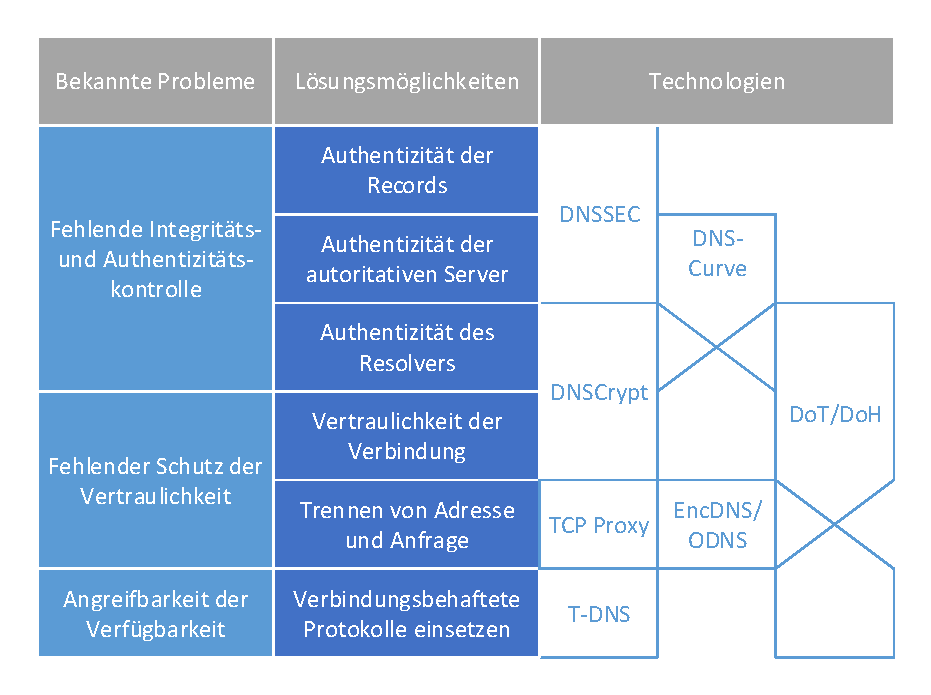
\includegraphics[width=0.7\textwidth]{Overview_Tecs}
    \caption{Darstellung des Bezugs zwischen DNS-Security Problemen, Lösungsmöglichkeiten und den bestehenden Technologien zur Umsetzung der Lösungen}
    \label{img:technologies-summary}
\end{figure}